\documentclass[{../../master}]{subfiles}
\graphicspath{{../..}}  % 個別コンパイル時の画像パスを解決する

\begin{document}

\section{\textsf{base\_link}の作成と追加}

節\ref{sec:create_urdf_package}までの作業で,ルートファイル\textsf{robot.xacro}の作成と\textsf{base\_footprint}リンクの定義を行いました.
この節ではロボットのボディのリンクである\textsf{base\_link}の定義とルートファイルへの追加の作業を行います.

\subsection{\textsf{base.xacro}の作成}

まず,\textsf{base\_link}の要素や属性の定義を記述するファイルを作成します.
\textsf{urdf/}ディレクトリ以下に\textsf{base/}ディレクトリを作成し,\textsf{base.xacro}という名前のファイルを作成します.
そして,まずはコード\ref{code:base_link_first_step}のような内容を記述します.

\begin{lstlisting}[language=XML, caption=\textsf{base.xacro}, label=code:base_link_first_step]
<?xml version="1.0"?>
<robot xmlns:xacro="http://ros.org/wiki/xacro">
  <xacro:macro name="base" params="parent *joint_origin">
    
  </xacro:macro>
</robot>
\end{lstlisting}

ルートファイルと同じく,\textsf{robot}タグをトップレベルに記述し,その中に他の全ての要素を記述していきます.
ただし,コンポーネントファイルには\textsf{name}属性を書く必要はありません.名前空間だけ指定しておきましょう.

\textsf{robot}タグの中には,\textsf{xacro:macro}タグが書かれています.
これが\textsf{xacro}におけるマクロの定義であり,ルートファイルから呼び出されるものです.
マクロの中に\textsf{link}や\textsf{joint}等のタグを記述しておけば,ルートファイルから呼び出されたときにそれらが展開される,という仕組みです.
\textsf{xacro:macro}タグには\textsf{name}属性と\textsf{params}属性があります.
\textsf{name}属性にはマクロの名前を指定します.
\textsf{params}属性には,そのマクロが取る引数を指定することができます.
引数は複数設定することができ,半角スペースで区切って記述します.
コード\ref{code:base_link_first_step}では,引数として\textsf{parent}(親リンク名の指定)と\textsf{*joint\_origin}
\footnote{アスタリスクが先頭に付くパラメータは「ブロックパラメータ」と呼ばれるパラメータで,任意の要素を展開することができます.}
(座標原点の指定)の2つを取るように設定しています.

\textsf{base.xacro}ファイルでは,このマクロを読み込んだら「\textsf{base\_link}の定義」と「\textsf{base\_footprint}と\textsf{base\_link}を繋ぐジョイント\textsf{base\_link\_joint}の定義」が行われるようにマクロを定義します.

\subsection{\textsf{joint}の設定}

この小節では\textsf{base\_link\_joint}の定義を行います.
コード\ref{code:base_link_joint_configuration}のようにマクロタグ内に\textsf{joint}タグを追記します.

\begin{lstlisting}[language=XML, caption=Configurate \textsf{base\_link\_joint}, label=code:base_link_joint_configuration]
<?xml version="1.0"?>
<robot xmlns:xacro="http://ros.org/wiki/xacro">
  <xacro:macro name="base" params="parent *joint_origin">
    <joint name="base_link_joint" type="fixed">
      <xacro:insert_block name="joint_origin"/>
      <parent link="${parent}"/>
      <child link="base_link"/>
    </joint>
  </xacro:macro>
</robot>
\end{lstlisting}

\textsf{joint}タグは\textsf{name}と\textsf{type}の2つの属性を持ち,また以下の要素を持ちます.\cite{urdf_xml_joint}

\begin{itemize}
  \item \textsf{origin}:親リンクから見たジョイントの原点座標
  \item \textsf{parent}:親リンク名
  \item \textsf{child}:子リンク名
  \item \textsf{axis}:ジョイントの軸.回転ジョイントの場合は回転軸を表す
  \item \textsf{calibration}:ジョイントの絶対位置を校正するために使用される,ジョイントの基準位置
  \item \textsf{dynamics}:ジョイントの物理的特性を指定するための要素
  \item \textsf{limit}:ジョイントの角度,力,速度のリミットを指定するための要素
  \item \textsf{mimic}:他のジョイントの動きを真似させるときに使用する要素
  \item \textsf{safety\_controller}:ジョイントが安全に動作するために設定するソフトなリミット
\end{itemize}

\noindent
このうち,ジョイントの定義に必須なのは\textsf{parent}と\textsf{child}のみで,他の要素は指定しなくてもジョイントを定義することができます.

ここでは,ジョイント名を「\textsf{base\_link\_joint}」,ジョイントタイプを「\textsf{fixed}」とし,要素には\textsf{parent}と\textsf{child},そして\textsf{origin}を設定します.

\textsf{child}要素は\textsf{base\_link}です.
\textsf{base\_link}はまだ存在せず,\ref{sec:base_link_define_link_tag}で定義します.
\textsf{parent}要素にはマクロが引数として受け取った値をそのまま使用します.
引数をマクロ内で利用するには,\textsf{\$\{\<PARAMETER\_NAME\>\}}の書式を使用します.

\textsf{joint}タグの\textsf{origin}要素で指定するのは,親リンクから見たジョイントの原点座標です.
図\ref{fig:joint}のように,ジョイントが子リンクの原点になります.
ここでは\textsf{base\_link}が子リンクなので,\textsf{base\_link}の座標系原点は\textsf{base\_link\_joint}の位置になるという事になります.

\begin{figure}[ht]
  \centering
  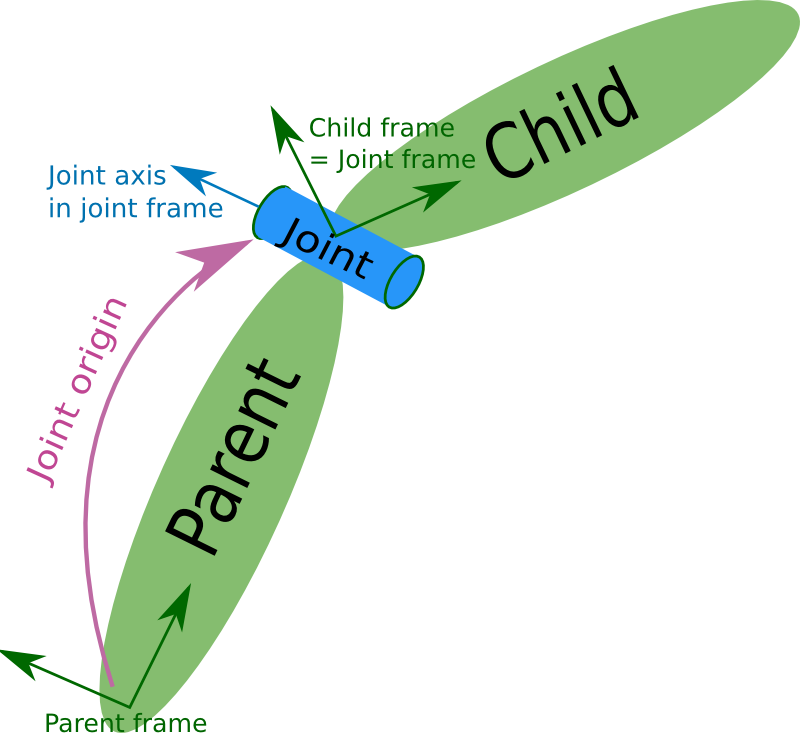
\includegraphics[width=100truemm, clip]{images/joint.png}
  \label{fig:joint}
  \caption{Coordinate Transformation Relationship Between Link and Joint\cite{urdf_xml_joint}}
\end{figure}

\textsf{origin}要素もマクロが引数として受け取ったものを使用します.
ただし,\textsf{origin}要素は単なる値ではないため,\textsf{parent}要素のようにそのまま使うことはできません.
そこで使用するのがブロックパラメータと呼ばれる引数です.
これを使用することで,ルートファイルからジョイントの\textsf{origin}要素を定義できるようになります.
コード\ref{code:base_link_joint_configuration}では\textsf{*joint\_origin}という名前でブロックパラメータを定義しています.
ルートファイルから読み込む際の詳細は\label{sec:base_link_include}で説明します.

ジョイントの設定は以上で完了です.次は\textsf{link}タグの設定を行います.

\subsection{\textsf{link}タグの設定}
\label{sec:base_link_define_link_tag}

\textsf{base\_link}の要素を記述していきます.
\textsf{link}タグは\textsf{inertial},\textsf{visual},\textsf{collision}の3つの要素を持ちます.
以下の小小節でそれぞれのタグを設定していきます.

\subsubsection{\textsf{visual}要素の定義}

まずは\textsf{visual}要素を記述しましょう.
\textsf{visual}要素はモデルの見た目の要素を定義するタグです.
コード\ref{code:link_element}のようにマクロタグ内に\textsf{link}タグを追記し,更にその中に\textsf{visual}要素を記述します.

\begin{lstlisting}[language=XML, caption=\textsf{link} Element, label=code:link_element]
<?xml version="1.0"?>
<robot xmlns:xacro="http://ros.org/wiki/xacro">
  <xacro:macro name="base" params="parent *joint_origin">
    <link name="base_link">
      <visual>
        <origin xyz="0.0 0.0 0.0"/>
        <geometry>
          <mesh filename="package://adamr2_description/meshes/base_link.STL"/>
        </geometry>
        <material name="red">
          <color rgba="1.0 0.0 0.0 1.0"/>
        </material>
      </visual>
    </link>
  </xacro:macro>
</robot>
\end{lstlisting}

\subsection{メッシュファイル(STL形式)の作成と割り当て}



\subsection{ファイルのインクルード}
\label{sec:base_link_include}

\subsection{\textsf{rviz}による可視化}

\end{document}